\documentclass[a4paper, 11pt, oneside]{article}
\usepackage[svgnames]{xcolor}
\usepackage{graphicx} % Required for box manipulation
\usepackage{geometry}
\usepackage{pgfplots}
\pgfplotsset{compat=1.14}
\geometry{legalpaper, margin=1in}
\newcommand*{\plogo}{\fbox{$\mathcal{PL}$}} % Generic dummy publisher logo

\usepackage[utf8]{inputenc} % Required for inputting international characters
\usepackage[T1]{fontenc} % Output font encoding for international characters
\usepackage{PTSerif} % Use the Paratype Serif font
\usepackage{amsmath}
\usepackage{amssymb}



\begin{document}

\begin{titlepage} % Suppresses headers and footers on the title page

	\centering % Centre all text
	
	%------------------------------------------------
	%	Title and subtitle
	%------------------------------------------------
	
	\setlength{\unitlength}{0.6\textwidth} % Set the width of the curly brackets above and below the titles
	
	{\color{LightGoldenrod}\resizebox*{\unitlength}{\baselineskip}{\rotatebox{90}{$\}$}}}\\[\baselineskip] % Top curly bracket
	
	\textcolor{Sienna}{\textit{\Huge MAST90045\\ $\;$ \\Systems Modelling and Simulation}}\\[\baselineskip] % Title
	
	{\color{RosyBrown}\Large Assignment 1}\\ % Subtitle or further description
	
	{\color{LightGoldenrod}\resizebox*{\unitlength}{\baselineskip}{\rotatebox{-90}{$\}$}}} % Bottom curly bracket
	
	\vfill % Whitespace between the title and the author name
	
	%------------------------------------------------
	%	Author
	%------------------------------------------------
	
	{\Large\textbf{Chris Swan 370502}}\\ % Author name
	
	\vfill % Whitespace between the author name and the publisher logo
	
	%------------------------------------------------
	%	Publisher
	%------------------------------------------------
	
	%\plogo\\[0.5\baselineskip] % Publisher logo
	
	University of Melbourne % Publisher name

\end{titlepage}

\tableofcontents

\newpage
\section{Problem Introduction}

This problem offers insight not only into applications of modelling and simulation, but also into methods for finding solutions to real world problems. Being able to accurately anticipate 
how rainfall will affect the level and volume of a dam is pertinent across the world. \\


But this is only a snapshot of the extensive applications that iterative modelling opens up.
The ability to find and offer solutions to problems that cannot be solved analytically is a valuable resource in business, industry and the wider community.  We therefore consider the 
exploration below as a reconnoitring of how iterative modelling can be used in these fields.\\

In this scenario we examine how change in volume affects the level of water in a dam. Whilst we begin by examining generic cases, we go on to examine more specific cases, with the goal of eventually being able to generalise for any scenario where certain information about a dam is known. In our specific case, our program developed below allows one to be able to extrapolate a change in the water level of a dam over time if the rainfall in the catchment area is known.

\section{Volume}

For any generic dam, we are given the function $A(h)$ to describe the cross-sectional area of the dam at height $h$.  We can then easily deduce that the volume of water contained within the dam
will be the integral of $A(h)$ with the limits (it being a 3-dimensional physical space) being from $0$ to $h$.  \\

We therefore have the volume function:

$$V(h) = \int_0^h A(u) \; du$$

As we want to be able to calculate $V(h)$ for any generic area function $A(h)$, we need some numerical algorithm for calculating the integral of $A(h)$ should it not be feasible (or possible) to solve $\int A(h)$ analytically.\\

Therefore, we elect to use Simpson's rule as our numerical algorithm for approximating $V(h)$. There are disadvantages in using approximation algorithms, as a precise answer cannot necessarily be computed, and Simpson's rule is no exception. However, in giving due consideration to the error that might result, Simspon’s rule will offer accuracy to a degree that any resulting error will be negligible.\\

Regarding the accuracy, through consideration of both the potential impact of approximation error as well as computation feasibility, we eventually elected to allow for an error tolerance of $1 \cdot 10^{-10}$ as balance between these two aspects.  Given that the units of area and volume are unknown, were the volume measured in Megalitres for example, a volume accuracy of $1\text{e}-10$ would give an accurate volume to 0.1 millilitres.  \\

Whilst this might seem excessive, accuracy to a ten-thousand-millionth of a megalitre allows for some flexibility should other models be required.  It was also computationally feasible for our model, and it should be noted that increasing the error tolerance increased the computation time of our root-finding algorithm significantly.  Given our discussion above, any further increase in accuracy was deemed unnecessary.\\

A further outline of the volume function and Simpson's rule can be found in Appendix B.

\section{Height}

Given a current level of the water in the dam $h$, we want to be able to calculate what the new dam level (or "height") will be for some change $v$ in the volume in the dam.  The new "height" will therefore be

$$u = H(h,v)$$

where $u$ satisfies

$$V(u) = V(h) + v$$

where $0 \leq V(u) \leq V(h_{\text{max}})$.  \\

If $V(u) < 0$, then $u = 0$ and if $V(u) > V(h_{\text{max}})$, then $u = h_{\text{max}}$.\\

Consequently, we need to define a new function that links these different constraints together and allows us to calculate values of $u$. To do this, we need to transform our function so that when $u$ is inputted, it returns a value of $0$.
This will allow us to make use of a root finding algorithm to compute $u$, which will be the value of the new height of the water in the dam after the change in volume.\\

For a root finding algorithm, we employ the Newton-Raphson method of using the derivative of a function to iteratively step towards its root. The concern with the Newton-Raphson method is that a function must be continuous and have a derivative $\in \mathbb{R}$ as the method involves dividing by the derivative. However, given that this derivative will be our area function, we can be assured that the derivate both exists and is well defined for $V(u)$ \\

In setting the tolerance and determining the number of iterations to run for the Newton-Raphson function, we explored a similar process to that used for Simpson's rule. In attempting to marry accuracy and efficiency, we found that unless the tolerance for the Simpson's function was excessively small, then convergence occurred relatively quickly with the Newton-Raphson tolerance set at a similar level ($10^{-10}$). \\


Setting the tolerance for the Newton-Raphson function smaller led to longer convergence, such that more than 100 iterations were needed, and making it even smaller ($\leq 10^{-14}$) saw the algorithm failing to converge in $10^{4}$ iterations. In consequence, we came to a similar deduction as we did with Simpson’s Rule, that a tolerance of $10^{-10}$ adequately covered variance in units bases for "height" without sacrificing computation time.\\

\section{Test Case}

The test case offered a good opportunity to troubleshoot and debug the program written, as well as refine our code to improve readability of output as well as the code itself. Augmenting additional functions proved useful for reuse later, as well as simplifying redundant or inefficient segments of code.\\

The testing of the functions, the output of which is shown in Figure 1, verified that our functions were acting correctly for values outside of the specified range, in this case returning NA for $h$ values outside of $0 \leq h \leq h_{\text{max}}$
and limiting the values of the new height, "dam\_level", at these values when they are returned outside of the specified range. Figure 2 gives some data visualisation of the values returned from the test inputs.

\newpage
\begin{figure}
\centering
\begin{tabular}{|c|c c c|}
\hline
Test Cases &Height Inputs&Volume Inputs&Height Outputs\\
\hline
1   & -1.0  &     1     &      NA\\
2  &   0.5  &     1    & 1.5000000000\\
3   &  0.5    &  -1   &  0.0000000000\\
4   &  3.5    &   1   &  3.7749172176\\
5   &  3.5     &  2  &   4.0000000000\\
6   &  3.5     & -1 &    3.2015621187\\
7  &   5.0     &  1   &        NA\\
\hline
\end{tabular}
\centering

\caption{Table of test case and results}
\end{figure}


\begin{figure}
\centering
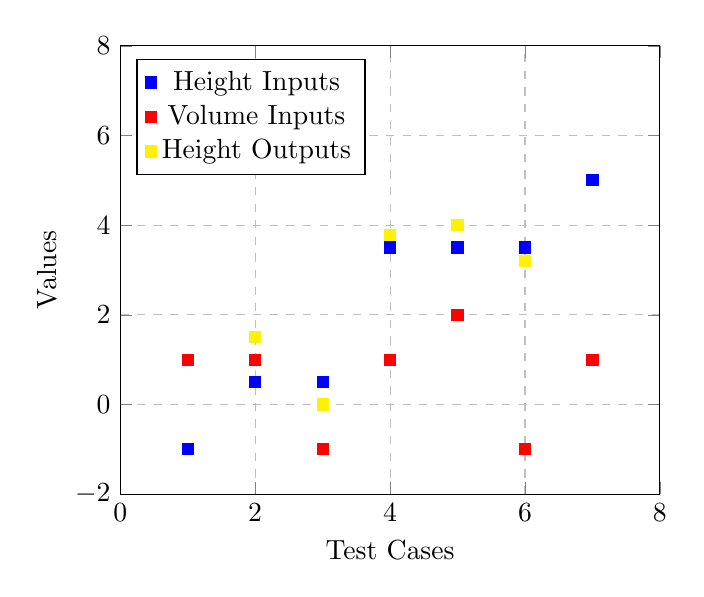
\begin{tikzpicture}
\begin{axis}[
xlabel={Test Cases},
ylabel={Values},
xmin=0, xmax=8, 
ymin=-2, ymax=8,
xmajorgrids=true,
ymajorgrids=true,
grid style=dashed,
legend pos = north west
]
\addplot[only marks, blue, mark=square*] table [x=a, y=e, col sep=comma] {
a,e
1,-1
2,0.5
3,0.5
4,3.5
5,3.5
6,3.5
7,5
};
\addlegendentry{Height Inputs}
\addplot[only marks, red, mark=square*] table [x=a, y=i, col sep=comma] {
a,i
1,1
2,1
3,-1
4,1
5,2
6,-1
7,1
};
\addlegendentry{Volume Inputs}
\addplot[only marks, yellow, mark=square*] table [x=a, y=j, col sep=comma] {
a,j
2,1.5
3,0
4,3.774917
5,4
6,3.201562
};
\addlegendentry{Height Outputs}
\end{axis}
\end{tikzpicture}
\caption{Results of test cases}
\centering
\end{figure}

\section{Tracking height over time}

We come to the implementation of what we have developed above. We have developed a method for calculating what the dam's height will be, based on the volume of rain falling in the catchment area, the volume of water used from the dam and the volume of water evaporated from the dam. The new level of water in the dam is thus given by

$$h(t+1) = H(h(t),v(t) - \alpha - \beta A (h(t)))$$

The area of the dam is defined by

\begin{flalign*}
A(h) &= 
\begin{cases}
	100h^2 \quad \quad &0 \leq h \leq 2\\
	400(h-1) \quad \quad &2 \leq h \leq 3
\end{cases}
\end{flalign*}

From this information, we can iteratively calculate the level of the dam after the volume of catchment water has been added.  \\




\begin{figure}
\centering
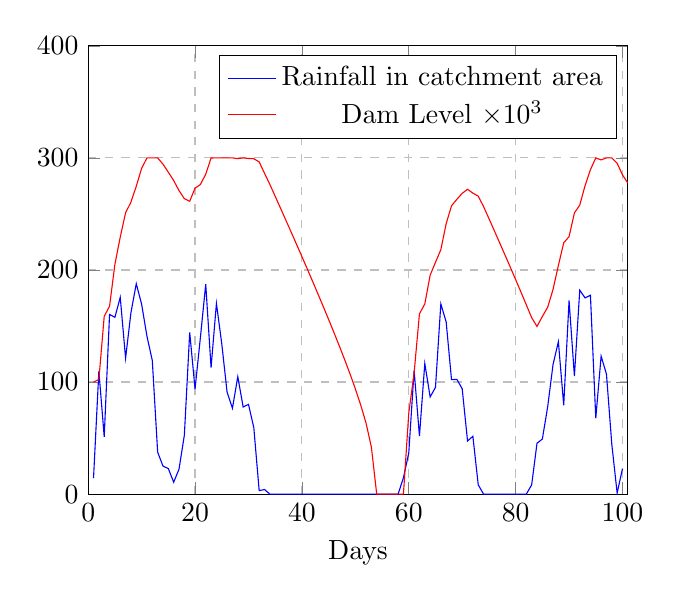
\begin{tikzpicture}
\begin{axis}[
xlabel={Days},
xmin=0, xmax=101, 
ymin=0, ymax=400,
xmajorgrids=true,
ymajorgrids=true,
grid style=dashed
]
\addplot[blue] table [x=a, y=e, col sep=comma] {
a,e
1,14.31711
2,109.8815
3,51.14796
4,160.3442
5,157.7805
6,175.575
7,121.2473
8,161.8492
9,187.721
10,169.4947
11,140.8879
12,119.2
13,37.49091
14,25.01957
15,22.7982
16,10.62324
17,22.28223
18,52.6329
19,144.3477
20,93.8219
21,139.6688
22,187.2834
23,112.8247
24,170.1796
25,134.1929
26,90.87007
27,76.63679
28,104.829
29,77.77952
30,80.05338
31,59.25845
32,3.165104
33,4.118153
34,0
35,0
36,0
37,0
38,0
39,0
40,0
41,0
42,0
43,0
44,0
45,0
46,0
47,0
48,0
49,0
50,0
51,0
52,0
53,0
54,0
55,0
56,0
57,0
58,0
59,14.57985
60,36.72097
61,110.4422
62,51.784
63,116.5769
64,86.67932
65,95.27534
66,169.7252
67,153.6469
68,102.1357
69,102.4133
70,93.9651
71,47.40445
72,51.57885
73,8.300242
74,0
75,0
76,0
77,0
78,0
79,0
80,0
81,0
82,0
83,8.257363
84,45.41098
85,49.1152
86,78.02648
87,115.5585
88,136.0315
89,79.32947
90,172.7445
91,105.3199
92,181.9667
93,175.0501
94,177.4771
95,67.73758
96,123.1144
97,107.1043
98,44.44291
99,0.9399437
100,22.811
};
\addlegendentry{Rainfall in catchment area}
\addplot[red] table [x=a, y=i, col sep=comma] {
a,i
1,100
2,102.265402
3,158.637015
4,167.6455069
5,205.0305921
6,229.3052143
7,251.0380222
8,260.4808048
9,274.7481978
10,290.5991046
11,300
12,300
13,300
14,294.356748
15,287.1854402
16,279.8182144
17,270.7904797
18,263.6083429
19,261.3293774
20,272.9681053
21,276.2092459
22,285.4965052
23,299.9079621
24,300
25,300
26,300
27,300
28,299.3284714
29,300
30,299.4717424
31,299.2541346
32,296.418049
33,286.3060498
34,276.3228029
35,265.7204718
36,255.0769659
37,244.3860313
38,233.6398346
39,222.8283709
40,211.9385603
41,200.9528112
42,189.8562931
43,178.6533866
44,167.3234195
45,155.8388262
46,144.1622558
47,132.2413381
48,119.9993787
49,107.3174152
50,93.9955787
51,79.6553791
52,63.4184257
53,42.0599025
54,0
55,0
56,0
57,0
58,0
59,0
60,72.2657042
61,108.0754685
62,160.8961618
63,169.6428973
64,195.360279
65,206.860191
66,218.0917592
67,241.3155632
68,257.2454201
69,263.058268
70,268.3671535
71,271.9837502
72,268.5495708
73,265.8822139
74,256.5703571
75,245.8864955
76,235.1485837
77,224.3469662
78,213.4690648
79,202.498036
80,191.4163045
81,180.2293983
82,168.9187063
83,157.4577494
84,149.5955562
85,158.4583454
86,166.7781085
87,182.5688131
88,204.0198922
89,224.2630884
90,229.7016841
91,250.8831276
92,257.8418532
93,275.3725993
94,289.4745407
95,300
96,298.2091799
97,300
98,300
99,295.2489321
100,284.8355054
101,277.5049406
};
\addlegendentry{Dam Level $\times 10^3$}
\end{axis}
\end{tikzpicture}
\caption{Volume of rain falling in catchment area and resulting dam level$\times 10^3$ }
\centering
\end{figure}


\section{Summary}

Creating a plot of the output of this (see Figure 3), we can clearly see the relationship that the rainfall has upon the level of water in the dam, as we expected. It is evident that there is some delay between a lack of rainfall and a drop in water level, and this itself provides opportunity for action were this model used to advise a body such a local or state government in a time of drought. \\

It is noteworthy that parts of this project can seem quite abstract when written in mathematical notation but have more clarity when explored iteratively. So too some aspects that are challenging to code are aided by exploring mathematical notation.\\










\newpage
\section{Apendices}
\subsection{Appendix A: Code}

\begin{verbatim}
rm(list=ls())

#spuRs alogorithms

# Simpson's Rule, taken from spuRs:
# program spuRs/resources/scripts/simpson.r

simpson <- function(ftn, a, b, tol = 1e-8, verbose = FALSE) {
  # numerical integral of ftn from a to b
  # using Simpson's rule with tolerance tol
  #
  # ftn is a function of a single variable and a < b
  # if verbose is TRUE then n is printed to the screen
  
  # initialise
  n <- 4
  h <- (b - a)/4
  fx <- sapply(seq(a, b, by = h), ftn)
  S <- sum(fx*c(1, 4, 2, 4, 1))*h/3
  S.diff <- tol + 1  # ensures we loop at least once
  
  # increase n until S changes by less than tol
  while (S.diff > tol) {
    # cat('n =', n, 'S =', S, '\n')  # diagnostic
    S.old <- S
    n <- 2*n
    h <- h/2
    fx[seq(1, n+1, by = 2)] <- fx  # reuse old ftn values
    fx[seq(2, n, by = 2)] <- sapply(seq(a+h, b-h, by = 2*h), ftn)
    S <- h/3*(fx[1] + fx[n+1] + 4*sum(fx[seq(2, n, by = 2)]) +
                2*sum(fx[seq(3, n-1, by = 2)]))
    S.diff <- abs(S - S.old)
  }
  if (verbose) cat('partition size', n, '\n')
  return(S)
}


# program spuRs/resources/scripts/newtonraphson.r
# loadable spuRs function

newtonraphson <- function(ftn, x0, tol = 1e-9, max.iter = 100) {
  # Newton_Raphson algorithm for solving ftn(x)[1] == 0
  # we assume that ftn is a function of a single variable that returns
  # the function value and the first derivative as a vector of length 2
  #
  # x0 is the initial guess at the root
  # the algorithm terminates when the function value is within distance
  # tol of 0, or the number of iterations exceeds max.iter
  
  # initialise
  x <- x0
  fx <- ftn(x)
  iter <-  0
  
  # continue iterating until stopping conditions are met
  while ((abs(fx[1]) > tol) && (iter < max.iter)) {
    x <- x - fx[1]/fx[2]
    fx <- ftn(x)
    iter <- iter + 1
    cat("At iteration", iter, "value of x is:", x, "\n")
  }
  
  # output depends on success of algorithm
  if (abs(fx[1]) > tol) {
    cat("Algorithm failed to converge\n")
    return(NULL)
  } else {
    cat("Algorithm converged\n")
    return(x)
  }
}


######################################################################################################

#volume
  

volume = function(h,hmax,ftn) {
  #we have function 'ftn' as the cross-sectional area of at height 'h', 
  #with 'hmax' as the max height
  if (h < 0) {
    return(NA)
  } else if (h > hmax) {
    return(NA)
  } else {
    V = simpson(ftn,0,h, tol = 1e-10)
    return(V)
  }
}

#height
  
height = function(h,hmax,v,ftn) {
  #our function for computing the new dam level from a given current height 'h', 
  #the maximum dam level 'hmax',
  #the current volume 'v' and the area function 'ftn'
  if (h < 0) {
    return(NA)
  } else if (h > hmax) {
    return(NA)
  } else {
    new_volume = as.numeric(volume(h, hmax, ftn) + v)
    max_volume = volume(hmax,hmax,ftn)
    if (new_volume > max_volume) {
      dam_level = hmax
      print(cat('The dam has reached the maximum level of', dam_level, '\n'))
    } else if (new_volume < 0) {
      dam_level = 0
      print(cat('The dam has reached the minimum level of', dam_level, '\n'))
    } else { 
      newt_input = function(x) {
        N = volume(x,hmax,ftn) - new_volume
        return(c(N,ftn(x)))
      }
    dam_level = newtonraphson(newt_input,hmax, tol = 1e-10, max.iter = 1000)
    }
  return(dam_level)
  }
}


#translating our variables to the assignment:

# dam_level = u = H(h,v)
# volume (function) = V(h)
# new_volume = V(u)
# ftn (function) = A(h)

######################################################################################################

#test case




heights = c(-1,0.5,0.5,3.5,3.5,3.5,5)
volumes = c(1,1,-1,1,2,-1,1)

# Let's evaluate our test criteria:

A = function(h) return(h)
V_h = function(k) return(k^2/2)
H_h_v = function(i,j) return(sqrt(i^2 + 2*j))

for (i in seq(1,7)) {
      print(cat("The Area of A", i," is ", A(heights[i]), "\n", 
                'The Volume of V', i," is ", V_h(heights[i]), "\n",
                'The Dam Level of H',i, " is ", H_h_v(heights[i],volumes[i]), "\n",
                'The New Height of h', i, " is ", height(heights[i],
		 hmax = 4, volumes[i], ftn = A), "\n"))
}

######################################################################################################


#tracking height over time

catchment = scan(file = "/School/Mast of Sci/MAST90045/A1/catchment_b-1.txt")

dam_calc = function(volume_data, initial_height = 1, hmax = 3, alpha = 2, beta = 0.1) {
  #our function for calculating the new levels of a dam from a vector of catchment data of
  #volume of rainfall, with 'volume_data' being a vector of catchment volume, 
  #'initial_height' being the starting dam level, 'hmax' being the max dam level,
  #'alpha' being the volume of water taken from the dam for use per day and
  #'beta' being the volume of water lost due to evaporation during a day
  h_vector = c(initial_height)
  len = length(catchment)
  Area = function(h) {
    if (0 <= h & h <= 2) {
      return(100*h^2)
    } else if (2 <= h & h <= 3){
      return(400*(h - 1))
    } else (
      return(NA)
    )
  }
  for (i in seq(1,len)) {
    if (h_vector[i] < 0) {
      h_vector[i] = 0
    } else if (h_vector[i] > hmax) {
      h_vector[i] = hmax
    } 
    vol = volume_data[i] - alpha - beta*Area(h_vector[i])  
    next_h = height(h_vector[i], hmax, vol, Area)
       
    h_vector = append(h_vector, next_h)
    
  } 
  return(h_vector)
}

rain_volumes = append(catchment, NA)
dam_heights = dam_calc(catchment)
dam_heights = formatC(dam_heights, digits = 10, format = 'f')
Results = cbind(rain_volumes,dam_heights)
write.csv(Results, file = "/School/Mast of Sci/MAST90045/A1/results.csv")

days = 1:101
plot(days,dam_heights, type="l")



\end{verbatim}

\newpage

\subsection{Appendix B: Functions \& Algorithms}

\subsubsection{Volume function and Simpson's rule}

$$S= \frac{y}{3}\bigg( f(x_0) + 4\sum_{i=1}^{n-1} f(x_{2i}) + 2\sum_{i=2}^{n-2} f(x_{2i}) + f(x_n) \bigg)$$

where $y$ is the difference between the limits of our integral, with $a$ being the lower limit and $b$ being the upper limit.  This is then divided by the number of partitions $n$.  $$\therefore y = \frac{b - a}{n}$$

\textbf{NB} $y$ is commonly notated as $h$ in Simpson's rule, but we call it $y$ to avoid confusion with our "height" variable  "h".\\

The sequence $[1,4,2,4, \cdot,4, 1]$ that can be observed is a method for saving on computational cost, enabling the algorithms to reuse previously computed values of $f$.  \\

The number of partitions $n$ will increase until S changes by less than the specified tolerance.\\

Our volume function calls Simpson's rule to evaluate the integral of our area function.

$$V(h) =  \frac{\frac{h - 0}{n}}{3}\bigg( A(x_0) + 4\sum_{i=1}^{n-1} A(x_{2i}) + 2\sum_{i=2}^{n-2} A(x_{2i}) + A(x_n) \bigg)$$

\subsubsection{Height function and the Newton-Raphson method}

The Newton-Raphson method for iteratively finding a root of a function $f(x)$ is defined as

$$x_{n=1} = x_n - \frac{f(x_n)}{f'(x_n)}$$

where $f'(x_n)$ is defined and not equal to 0.\\

From definition of volumes of the new dam level, we can see the following:

\begin{flalign*}
V(u) &= V(h) + v\\
0 &= V(u) - V(h) - v\\
&\frac{d}{du}\bigg(  V(u) - V(h) - v \bigg)\\
&= V'(u)\\
&= f(u)
\end{flalign*}

Therefore, we have all components necessary for computing roots of V(u).


\end{document}
